\documentclass[11pt,twocolumn]{article}
\usepackage{graphicx}
\usepackage[margin=1in]{geometry}
\usepackage{natbib}
\usepackage{amsmath, amssymb, graphicx}
\usepackage{authblk}
\renewcommand\Authfont{\normalsize}
\renewcommand\Affilfont{\small}
\setlength{\affilsep}{0pt}


\begin{document}

\title{\textbf{Recreating the 1967 Silicon Fuzz Face Circuit\\ with Additional Tone Control}}
\author{Brodie Monohan}
\author{Danny Sewell}
\affil{\textit{Whitman College}}
\affil{monohanb@whitman.edu}

\date{December 11, 2025}

\twocolumn[
\begin{@twocolumnfalse}
\maketitle

\begin{abstract}
The Germanium Fuzz Face and Silicon Fuzz Face are some of the most ubiquitous sounds in 1960s and 70s Rock n' Roll, named after the transistors used in them. The germanium transistor circuit was most famously used by Jimi Hendrix while the later silicon version was used by artists like David Gilmour. This is a particularly interesting circuit as its short parts-list betrays its complexity. One of the ways this circuit creates its unique sound is with intentionally poorly biased transistors that distort the signal lopsidedly. Our goal is to recreate this pedal circuit with more modern parts and add additional tone control which the original pedal was noticeably missing. We will focus on the later Silicon Fuzz Face as it used the more familiar NPN transistors rather than PNP\@.
\end{abstract}


\vspace{1cm}
\end{@twocolumnfalse}
]

\section{Introduction}

The original Silicon and Germanium Fuzz Face circuits consisted of two transistors in series that acted as common amplifiers. Over the 60 year run of these pedals' production, the transistors used in them included the NKT275, AC128, and SFT363E in the germanium circuits, and the BC108C, BC183L, BC109, BC109C, and BC209C in the silicon circuits. For the silicon circuits, these transistors have a $\beta$ of around 120. Other characteristics of these transistors effected the style of the distortion in each iteration, but any NPN Transistor (especially with a similar $\beta$) will work in this circuit to produce similar distortion magnitudes. This is because the amount of current it pulls through the collector terminal and the voltage rails determine the amount of amplification and clipping the transistors can impart on the signal. 

\begin{figure}
    \centering
    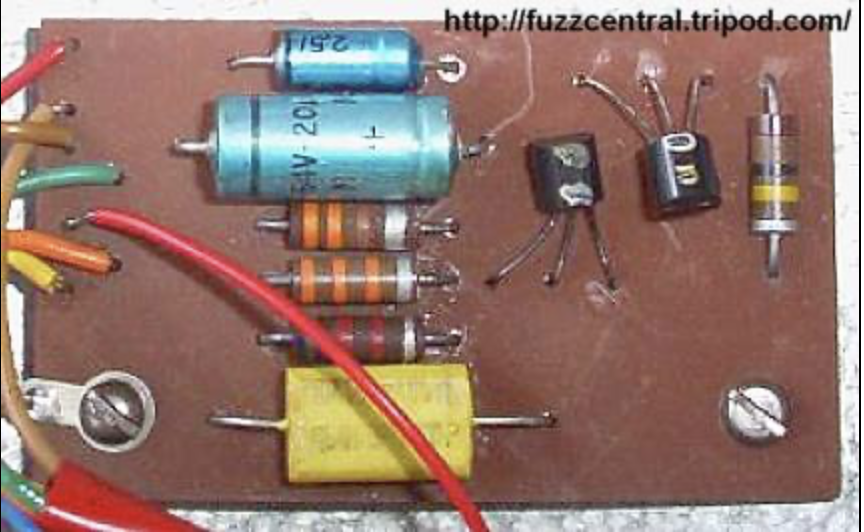
\includegraphics[width=1\linewidth]{../figures/original_im.png}
    \caption{An image of the PCB of the original 1967 Silicon Fuzz Face circuit}\label{fig:original_im}
\end{figure}
\begin{figure}
    \centering
    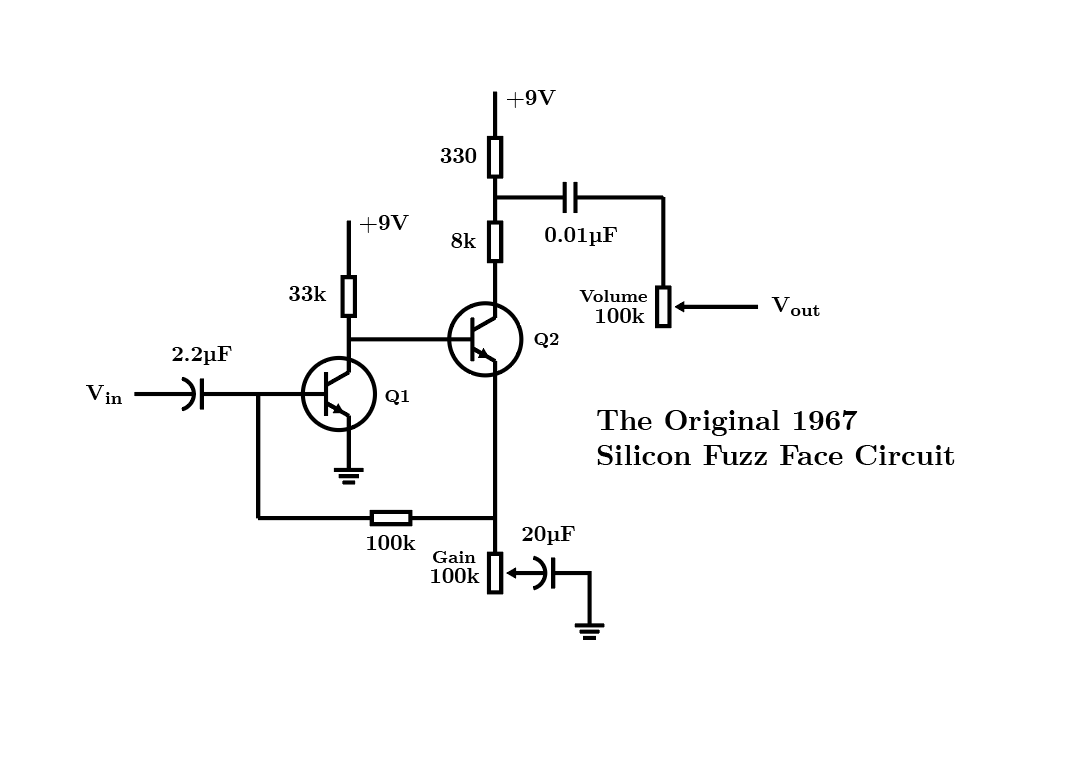
\includegraphics[width=1\linewidth]{../figures/original_dia.png}
    \caption{A schematic of the original Silicon Fuzz Face circuit from 1967 pieced together from images and resources online}\label{fig:original_dia}
\end{figure}

\begin{figure*}[t]
    \centering
    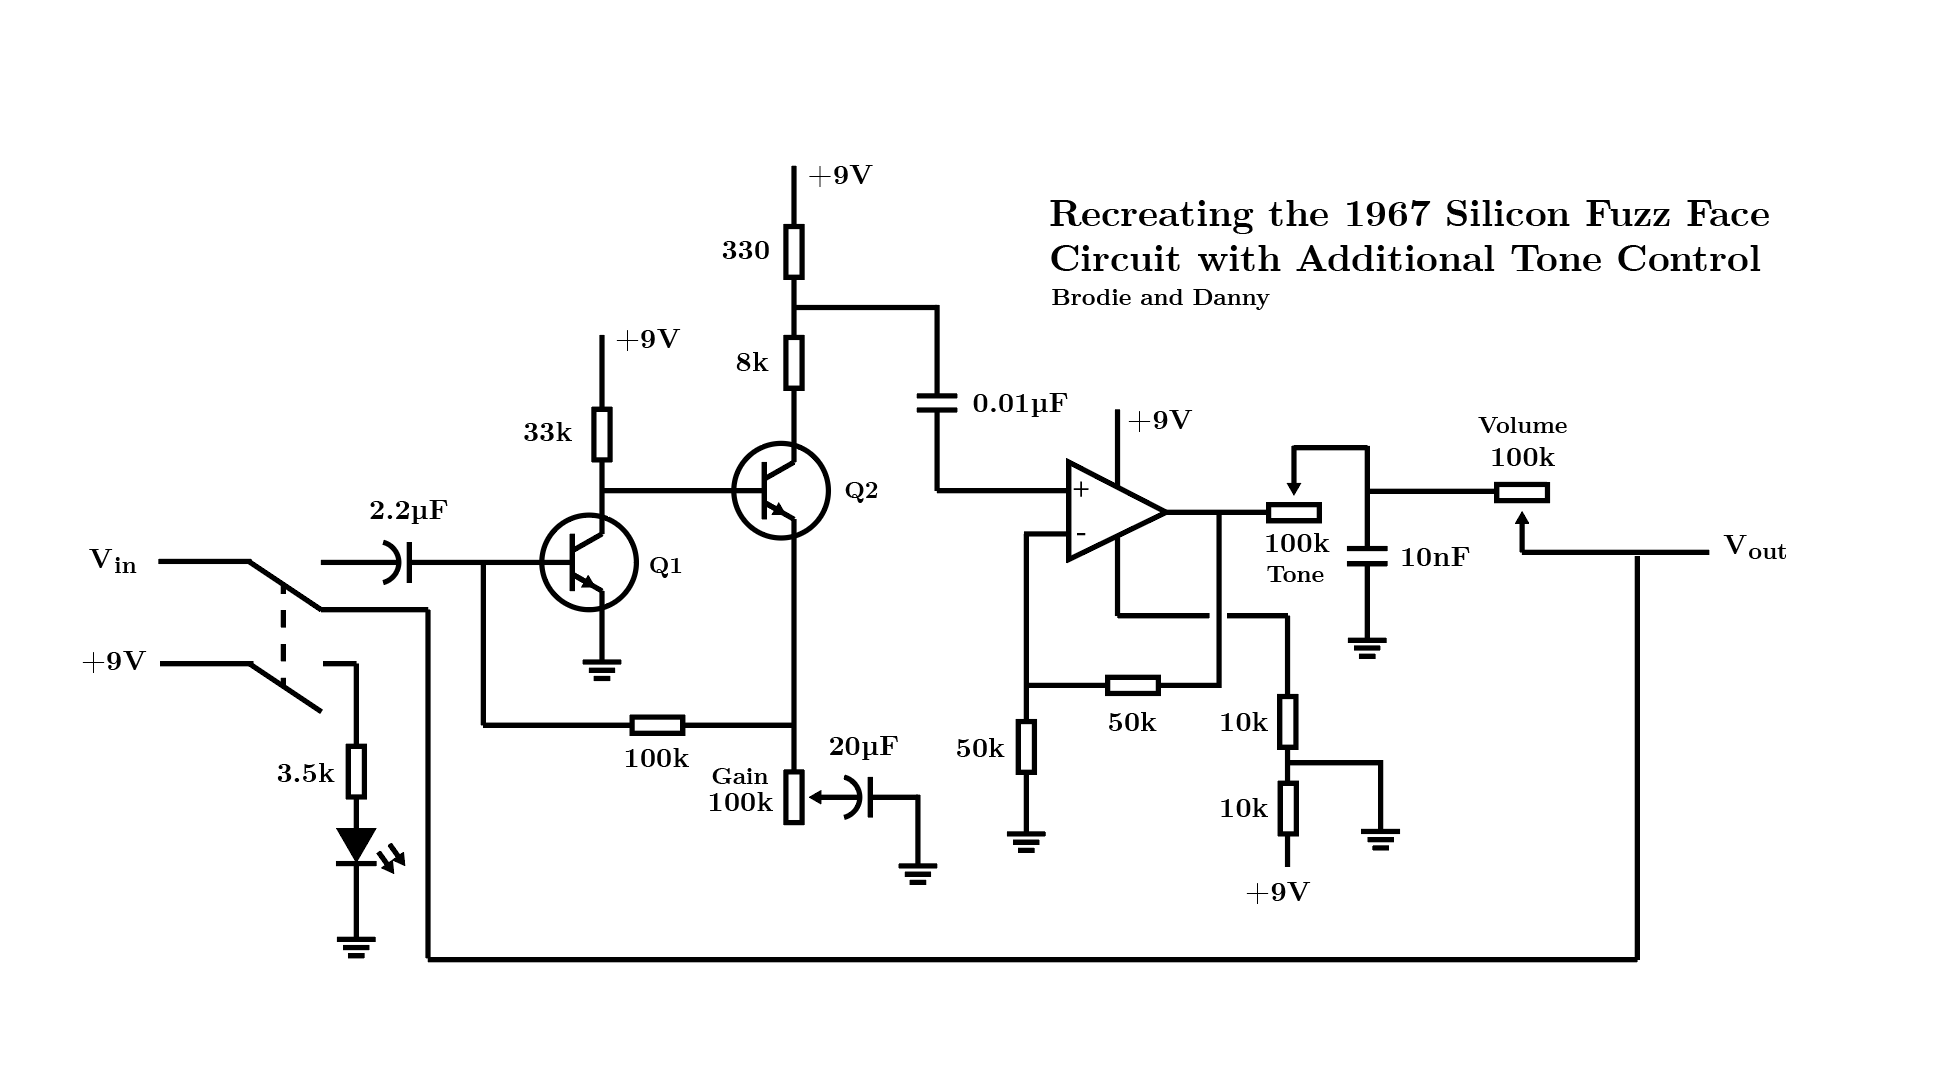
\includegraphics[width=\textwidth]{../figures/prelim_dia.png}
    \caption{A preliminary diagram of our modified Silicon Fuzz Face circuit with some of our best estimations for resistor values. We will likely need to build and test or simulate the circuit in Python or in some circuit simulation software to precisely determine the best resistor values for the transistor stages.}\label{fig:enter-label}
\end{figure*}

Figure 1 shows the circuit board of the original Silicon Fuzz Face from 1967, and Figure 2 shows the circuit design as a readable schematic (the value of the gain pot varies by online account, some have it as high as 100k and some as low as 1k). The first transistor in the Silicon Fuzz Face circuit is a buffer transistor, however, it is intentionally ``poorly'' biased. The DC operating point is near 1.2V which means the signal will be clipped more on the bottom than on the top. Some sources online also claim that low input impedance through the 100k feedback resistor is the reason this pedal is considered ``smooth'' with volume roll off because when the volume is turned down and the input impedance raises in tandem, the amount of interaction with the pickups comes down with it. In the original circuit, the first transistor Q1 has a collector resistor that is $\rm 33k\Omega$ and the emitter tied directly to ground. This means this stage has a huge gain because the emitter resistance is only the internal resistance of the transistor (order of magnitude $\rm A_v\approx -100$). However, guitar signals only range from about 10 mV to 1V peak to peak. With the low input impedance of the circuit, this will be attenuated even lower. This means while the gain is huge, there won't actually be that much clipping in this stage by itself. Only when the second transistor is attached and voltage from its emitter is fed back into the base of this transistor will the signal really start to distort. It is hard to know at this point how much the signal will be clipped and at what stage because all we have is a DC description of the circuit, but generally it seems clear that most of the clipping will happen in the second transistor. The second transistor has an operating point of 8.9V which is \textit{just} below the top rail (saturation will start at 9V). We will likely want this to be lowered when we build our circuit by reducing the collector resistor or increasing the 330$\Omega$ resistor (or both) considering this is very high and we anticipate a different $\beta$ from our transistors which we will need to adapt to. After the gain stages, the signal is passed through a $10$nF capacitor which cuts out some of the low end of the signal and the offset from the operating point near 9V and finally through a 100k pot for volume. 

\section{Our Plan for Modifications}
For our modifications and extensions we will break the circuit up into four main stages and one parallel stage for a power indicator LED\@. The stages are as follows:

\begin{enumerate}
    \item The high pass DC offset removal (just a high capacitance capacitor).
    \item The Q1 transistor which clips the bottom of the signal.
    \item The Q2 transistor which clips the top of the signal heavily (this stage feeds voltage back into the first transistor) and gain potentiometer.
    \item The low pass filter with a variable cutoff frequency (tone) and volume with potentiometers.
    \item The indicator LED which will trigger when the circuit is active and will turn off when the foot switch is in bypass mode.
\end{enumerate}

\begin{figure*}[t]
    \centering
    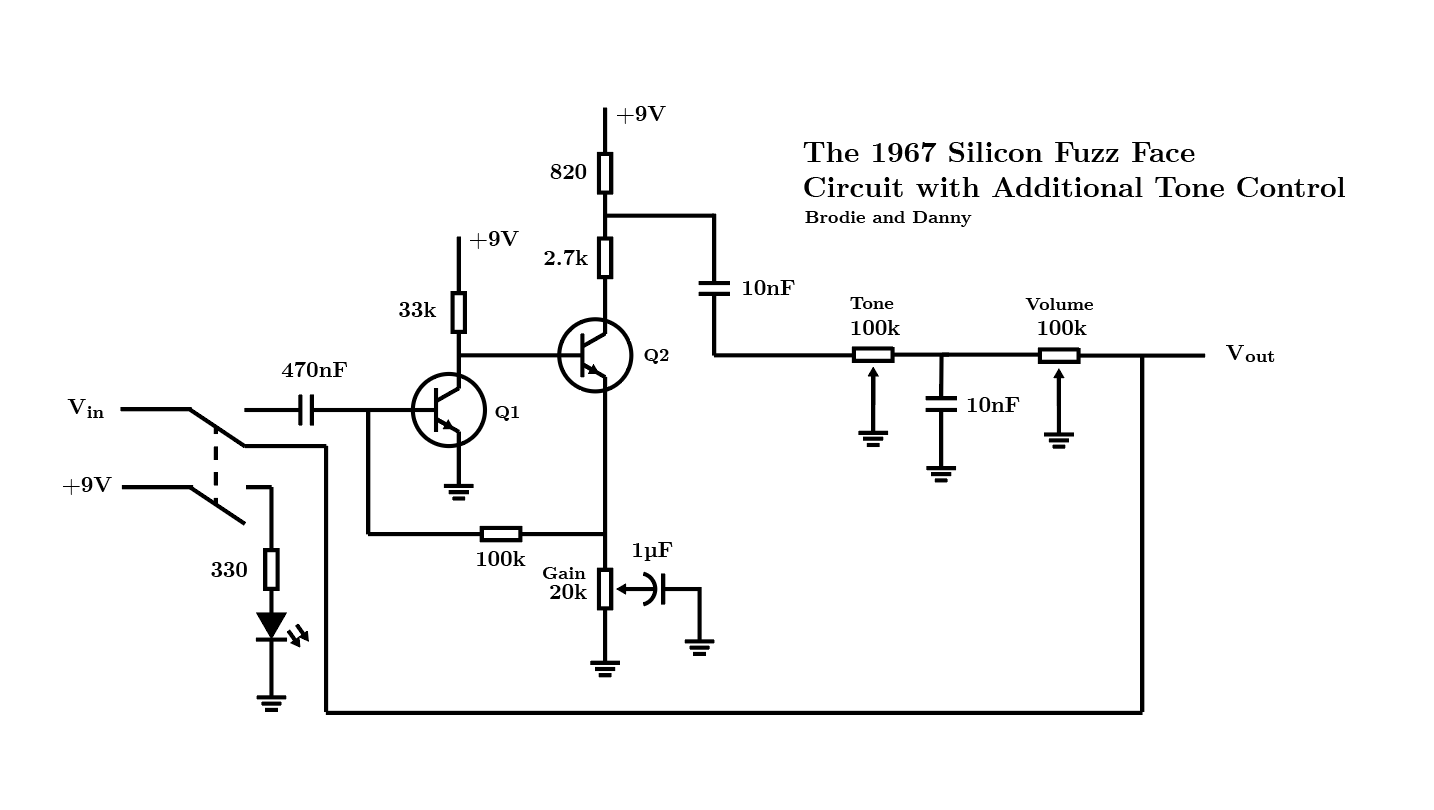
\includegraphics[width=\textwidth]{../figures/final_dia.png}
    \caption{The final modified Silicon Fuzz Face design.}\label{fig:final_dia}
\end{figure*} 

We will also need to consider hardware. We will need 2 NPN Transistors (BC108C, BC183L, BC109, BC109C, or BC209C) like the ones mentioned above. We will also need 2, 1/4 inch TS Panel-mount input jacks (11PKG) to get the input signal from a guitar and pass an output signal to an amp. We will need a 2.1mm 9V DC Power Jack to get 9V from a standard pedal power bank or cable. We will need a 9 Pin Foot Switch (060--078) to toggle between the circuit being active and a true bypass. We will need a couple electrolytic capacitors (20$\mu$F and 2.2$\mu$F if we follow the original exactly). Lastly, we will need an enclosure. The originals were housed in circular custom shaped enclosures but any metal enclosure will work for us. We elected for a cheap electrical box from Home Depot.

\subsection{The First Stage: Removing DC Offset}



The first thing we need to do is remove any DC offset coming from the guitar signal or any other circuits or processing before the signal comes into the Silicon Fuzz Circuit. A reasonably large capacitor should work to do this; something around $\rm C > 0.1\mu F$. This will act like a high pass filter with a cutoff frequency of $f_c > 1.6\rm Hz$. This capacitor is present in the original circuit as well (2.2$\mu$F) which has an even lower cutoff frequency.

\subsection{The Second Stage: The Buffer Transistor}

Like in the original, we will have a buffer transistor (we recognize this is a misnomer because there is still an impedance ``issue'') which will amplify this signal before the second transistor stage. By itself, it will do pretty much nothing to an incoming signal. This is because we removed all of the DC offset from the input (if there was any) and provide no voltage to the base (we would need $0.6$V). Typically we would use a voltage divider from the 9V supply for linear amplification. Only when we connect the second transistor stage does it get some base voltage through the feedback resistor. The DC operating point of the base terminal is 0.62V which is barely enough to turn it on. This means as an input signal swings low at some frequency greater than the cutoff point of the initial high pass filter, the bottoms will be cut off heavily while the tops will be likely unaffected (depends on $\beta$). The main function for this stage seems to be to cut the bottom half of the signal so that the second transistor can cut the top. We think the designers built it this way so that the asymmetry of the clipping, which we can control with the amount of current through the emitter of the second resistor, will create a unique distortion sound compared to equal clipping on the top and bottom of the signal.

\subsection{The Third Stage: The Saturation Transistor}

The output of the first transistor stage will lead into the base of the second transistor stage. This stage will not only amplify the signal again but will clip the top half this time with the DC operating point pulled very high (8.9V) which is dictated by the two collector resistors. We can also control the amount that the signal is chopped on the top with the amount of current that can pass through the emitter. With the gain pot fully open, the AC signal can just run to ground and the current allowed is maximum. With it fully closed the 100$k\Omega$ of resistance limits the amount of current that can flow. With the gain open, this all results in a heavily distorted signal that is uneven on the top and bottom, oscillating just below 9V. We will use another decently large capacitor here to bring this back to oscillating around 0V.

\subsection{The Fourth Stage: Tone and Volume}
\begin{figure}
    \centering
    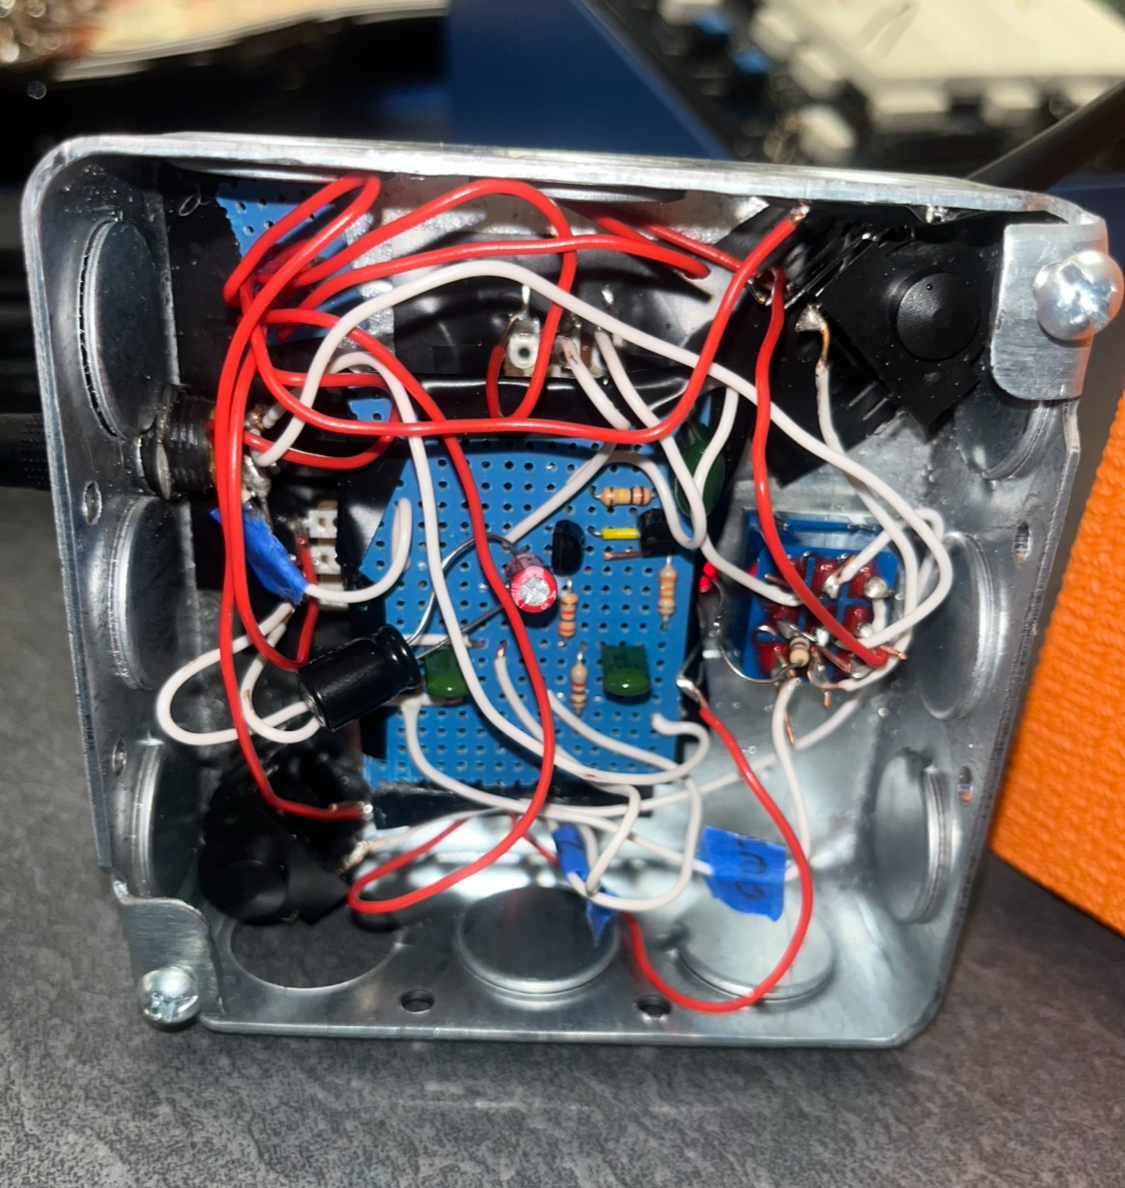
\includegraphics[width=1\linewidth]{../figures/final_im.jpg}
    \caption{An image of the final circuit in its enclosure.}\label{fig:final_im}
\end{figure}
First we will use a standard op-amp to prevent loading the initial stages with 9V rails. After that, the tone stage is just a 100k potentiometer as the resistor in a high-pass filter. The cutoff frequency scales as $1/R$ so as the resistance goes to 0 in the potentiometer, the cutoff frequency goes to infinity. When the potentiometer is fully closed the cutoff frequency will become $\approx \rm 16kHZ$. The volume is just a potentiometer that will dump the signal to ground when closed and let it all through to $\rm V_{out}$ when open.

\subsection{The LED Parallel Stage}

For the LED to be on it needs to have the correct resistor to limit current. If we want 20mA (nice and bright), then we can find the correct resistor with $R=V_{\rm cc}-V_{\rm forward}/I_{\rm LED} \rightarrow R=350\Omega\approx 330\Omega$.

\section{The Final Design}

The final circuit underwent some major changes. The first is the resistor values at the collector of Q2, which we expected to change. We used N2222 NPN silicon transistors, instead of those listed above from the original circuit, which have slightly different properties (mostly $\beta$) that we had to fine tune. The second is that we only had access to +9V and GND from the power input jack which means our op-amp needed to have rails at +9V and GND with a ground that it saw at 4.5V. This means we would need to impart a 4.5V offset on the signal before it entered the op-amp which came with some impedance issues that we never figured out. Instead, we let the tone stage load the collector resistors of Q2 which ended up helping with the over-clipping issues we knew we would have. We also changed the value of the gain capacitor based on sound testing. These changes can be found in Figure 4. Additionally, we had to connect two input jacks which required a ground each. We also had to wire the 9 pin foot switch. The layout of this switch, as well as our wiring and circuit board can be seen in Figure 5 (kind of).

\section{Errors and Potential Improvements}

Between testing the circuit outside of the box and putting it in, the amount of gain we were getting out changed quite a bit. We think there may have been a loose connection somewhere on the underside of the board, which, as you can see from Figure 5, was inaccessible once it was in. To compensate, we added a 330$\rm \mu F$ capacitor in parallel with the $\rm 1\mu F$ gain capacitor which seemed to work well. We also think that the gain pot is too large at 20k because it changes very fast before cutting the signal all the way out at about 80\% closed. We also soldered the volume and tone pots backwards so that a leftward turn is fully open and a rightward turn is fully closed (opposite of convention). In general, the soldering was quite poor (it was our first time) which means connections come apart frequently and loud pops come through the signal from jostles to the case. All of these would be easy fixes on a second try though and will be re-examined after this report. Otherwise the pedal works as it should and sounds good for quite inexpensive components and a design from over 50 years ago.

\end{document}